\documentclass[10pt,letterpaper]{article}
\usepackage[T1]{fontenc}
\usepackage{lmodern}
\usepackage{microtype}
\usepackage[letterpaper,top=.46in,bottom=.48in,left=.56in,right=.56in]{geometry}
\usepackage{xcolor}
\usepackage{tikz}
\usetikzlibrary{arrows.meta,calc,positioning}
\usepackage{multicol}
\usepackage{enumitem}
\usepackage{titlesec}
\usepackage{fancyhdr}
\usepackage[hidelinks]{hyperref}
\hypersetup{
  pdftitle={Private LLM inference, prepared before the prompt},
  pdfauthor={Blair Hudson},
  pdfsubject={PLLM public-weight prepared inference decision brief},
  pdfkeywords={private inference, prepared inventory, non-collusion}
}

\definecolor{pllmInk}{HTML}{112123}
\definecolor{pllmGreen}{HTML}{467A35}
\definecolor{pllmPale}{HTML}{E8EFE4}
\definecolor{pllmWarm}{HTML}{F2EBDD}
\definecolor{pllmLine}{HTML}{AAB9AC}
\definecolor{pllmMuted}{HTML}{506462}

\renewcommand{\familydefault}{\sfdefault}
\color{pllmInk}
\setlength{\parindent}{0pt}
\setlength{\parskip}{3.2pt}
\setlength{\columnsep}{.28in}
\setlist{nosep,leftmargin=1.2em,labelsep=.45em}
\setlist[itemize]{label=\textcolor{pllmGreen}{\rule{.38em}{.38em}}}
\setlist[enumerate]{label=\textcolor{pllmGreen}{\bfseries\arabic*.}}
\titleformat{\section}{\fontsize{12.4}{13.2}\selectfont\bfseries\color{pllmInk}}{}{0pt}{}
\titlespacing*{\section}{0pt}{7pt}{2pt}
\pagestyle{fancy}
\fancyhf{}
\renewcommand{\headrulewidth}{0pt}
\fancyfoot[L]{\fontsize{7}{8}\selectfont\color{pllmMuted} PLLM WHITEPAPER / REVISION 1.0}
\fancyfoot[R]{\fontsize{7}{8}\selectfont\color{pllmMuted} \thepage\ / 2}

\newcommand{\evidence}[1]{\textcolor{pllmGreen}{\bfseries\scriptsize #1}}
\newcommand{\refmark}[1]{\textsuperscript{\textcolor{pllmGreen}{[#1]}}}

\begin{document}
\thispagestyle{fancy}

\begin{minipage}[t]{.66\textwidth}
{\fontsize{8}{9}\selectfont\bfseries\color{pllmGreen}\MakeUppercase{Private inference / decision brief}}\\[5pt]
{\fontsize{26}{27}\selectfont\bfseries Private LLM inference,\\prepared before the prompt}\\[7pt]
{\fontsize{11}{14}\selectfont\color{pllmMuted} PLLM separates public-model computation across a customer client, trusted preparation service, and inference provider. Fresh one-time inventory moves preparation off the online path without removing its cost or trust assumptions.}
\end{minipage}\hfill
\begin{minipage}[t]{.28\textwidth}
\raggedleft\fontsize{8}{11}\selectfont
\textbf{Blair Hudson}\\
11 September 2026\\
Revision 1.0\\[7pt]
\color{pllmGreen}\textbf{CURRENT DESIGN}\\
\color{pllmMuted}Public-weight runtime\\
PLLM v0.17.0a1
\end{minipage}

\vspace{8pt}\textcolor{pllmLine}{\rule{\textwidth}{.6pt}}\vspace{5pt}

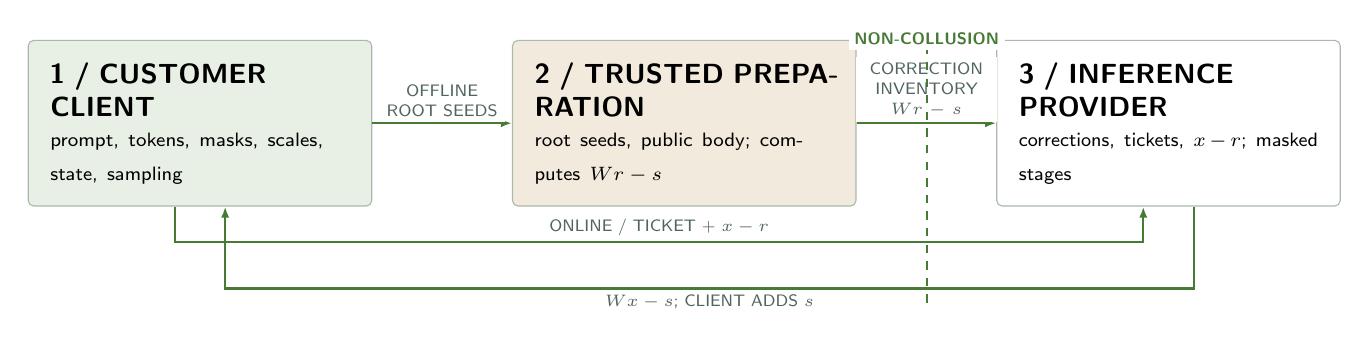
\begin{tikzpicture}[x=1cm,y=1cm,>=Latex,font=\sffamily]
  \tikzset{
    role/.style={draw=pllmLine,rounded corners=2pt,minimum height=1.45cm,align=left,inner sep=8pt},
    flow/.style={draw=pllmGreen,line width=.8pt,-{Latex[length=4pt]}},
    note/.style={font=\fontsize{6.4}{7.2}\selectfont,fill=white,inner sep=2pt,text=pllmMuted,align=center}
  }
  \node[role,fill=pllmPale,text width=3.80cm] (client) at (2.05,2.48) {\textbf{1 / CUSTOMER CLIENT}\\[-1pt]\fontsize{7.4}{8.4}\selectfont prompt, tokens, masks, scales, state, sampling};
  \node[role,fill=pllmWarm,text width=3.80cm] (prep) at (8.20,2.48) {\textbf{2 / TRUSTED PREPARATION}\\[-1pt]\fontsize{7.4}{8.4}\selectfont root seeds, public body; computes $W r-s$};
  \node[role,fill=white,text width=3.80cm] (infer) at (14.35,2.48) {\textbf{3 / INFERENCE PROVIDER}\\[-1pt]\fontsize{7.4}{8.4}\selectfont corrections, tickets, $x-r$; masked stages};
  \draw[flow] (client.east) -- node[note,above,text width=1.45cm] {OFFLINE\\ROOT SEEDS} (prep.west);
  \draw[flow] (prep.east) -- node[note,above,text width=1.65cm] {CORRECTION\\INVENTORY $Wr-s$} (infer.west);
  \coordinate (clientOnline) at ([xshift=-.32cm,yshift=-.45cm]client.south);
  \coordinate (inferOnline) at ([xshift=-.32cm,yshift=-.45cm]infer.south);
  \draw[flow] ([xshift=-.32cm]client.south) -- (clientOnline) -- node[note,above] {ONLINE / TICKET + $x-r$} (inferOnline) -- ([xshift=-.32cm]infer.south);
  \coordinate (inferReturn) at ([xshift=.32cm,yshift=-1.04cm]infer.south);
  \coordinate (clientReturn) at ([xshift=.32cm,yshift=-1.04cm]client.south);
  \draw[flow] ([xshift=.32cm]infer.south) -- (inferReturn) -- node[note,below] {$Wx-s$; CLIENT ADDS $s$} (clientReturn) -- ([xshift=.32cm]client.south);
  \draw[dashed,pllmGreen,line width=.8pt] (11.28,.20) -- (11.28,3.65);
  \node[font=\fontsize{6.4}{7}\selectfont\bfseries,text=pllmGreen,fill=white,inner sep=2pt] at (11.28,3.55) {NON-COLLUSION};
\end{tikzpicture}

\vspace{1pt}
\begin{multicols}{2}
\section*{What PLLM changes}
Ordinary hosted inference exposes prompts and generated text to one provider. PLLM instead keeps tokenization, nonlinear operations, attention state, sampling, and decoding in the customer environment. Public transformer-body matrices run remotely as masked integer projections. This is a deployment boundary, not a claim that an unmodified model API becomes private by changing its URL.\refmark{1}

\section*{Prepared inventory}
Before chat, the client commits an inventory to one model, body, stage set, quantization profile, and attempt budget. It sends one domain-separated root seed per stage to preparation. Preparation expands one-time input masks $r$, output masks $s$, and tickets, computes $Wr-s$, then pushes each batch to inference. Inference durably acknowledges every stage and seals the inventory \texttt{READY}. Online, it atomically consumes a ticket and returns
\[
W(x-r)+(Wr-s)=Wx-s.
\]
The client adds $s$. Prefill rows share a compact matrix envelope; decode retains one ticket per stage on a persistent connection. Unused reserved rows burn on cancellation or failure. Inventory is memory-only and disappears on restart or idle expiry.\refmark{1}

\section*{Boundary, not invisibility}
\textbf{Protected from inference:} plaintext prompts and outputs, token identities, root seeds, masks, activation scales, local attention and recurrent state, and sampling choices. Preparation sees seeds and bound stage metadata, but not online masked activations. Inference sees corrections and masked activations, but not seeds.

\textbf{Still exposed:} both services know the public model, stage names, tensor shapes, quantization profile, scheduling, timing, traffic volume, and approximate sequence lengths. Preparation must follow the protocol, erase expanded masks, and not collude with inference. Two services under one untrusted operator do not meet this assumption; authentication and TLS protect channels but do not prove independence, erasure, or correct model execution.\refmark{2}

Fresh uniform masks hide each online integer activation from inference when viewed alone. That claim is narrower than end-to-end confidential computing: it assumes protocol-conforming roles, keeps nonlinear work and state on the client, and does not verify provider execution. A network observer able to join both channels, a preparation service retaining masks, or colluding services can recover activation information. Deployment review must therefore name operators and log-access paths, not merely count endpoints.
\end{multicols}

\clearpage
\thispagestyle{fancy}

{\fontsize{8}{9}\selectfont\bfseries\color{pllmGreen}\MakeUppercase{Evidence and adoption gates}}\\[3pt]
{\fontsize{20}{22}\selectfont\bfseries Price the whole lifecycle, then decide.}

\vspace{7pt}
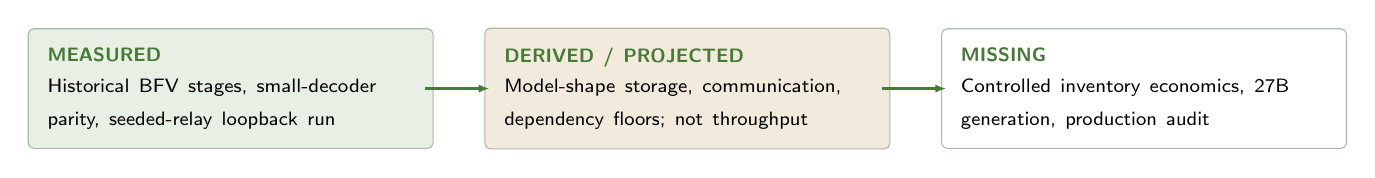
\begin{tikzpicture}[x=1cm,y=1cm,font=\sffamily]
  \tikzset{rung/.style={draw=pllmLine,rounded corners=2pt,minimum height=1.16cm,align=left,inner sep=7pt}}
  \node[rung,fill=pllmPale,text width=4.65cm] at (2.45,.65) {\evidence{MEASURED}\\[-1pt]\fontsize{7.2}{8.2}\selectfont Historical BFV stages, small-decoder parity, seeded-relay loopback run};
  \node[rung,fill=pllmWarm,text width=4.65cm] at (8.25,.65) {\evidence{DERIVED / PROJECTED}\\[-1pt]\fontsize{7.2}{8.2}\selectfont Model-shape storage, communication, dependency floors; not throughput};
  \node[rung,fill=white,text width=4.65cm] at (14.05,.65) {\evidence{MISSING}\\[-1pt]\fontsize{7.2}{8.2}\selectfont Controlled inventory economics, 27B generation, production audit};
  \draw[-{Latex[length=4pt]},pllmGreen,line width=.9pt] (4.92,.65) -- (5.74,.65);
  \draw[-{Latex[length=4pt]},pllmGreen,line width=.9pt] (10.72,.65) -- (11.54,.65);
\end{tikzpicture}

\vspace{2pt}
\begin{minipage}[t]{.485\textwidth}\vspace{0pt}
\section*{Economic cost ledger}
No repository evidence supports an ROI or savings percentage. A deployment model should count:
\begin{itemize}
  \item \textbf{Client:} local tokenization, nonlinear math, KV/recurrent state, public boundary matrices, memory, and model-plan transfer.
  \item \textbf{Preparation:} duplicate public body storage, mask expansion, matrix work, correction egress, secure erasure, and idle capacity.
  \item \textbf{Inference:} body storage, masked projection compute, inventory memory, online ingress/egress, and ticket bookkeeping.
  \item \textbf{Operations:} three credentials, TLS endpoints, telemetry, upgrades, replenishment, failures, and independent control of preparation.
\end{itemize}
Unit economics therefore depend on prompt shape, generated tokens, stage dimensions, concurrent demand, refill batch, burn rate, bandwidth price, and required operator separation.

\section*{Potential impact}
Offline preparation removes preparation round trips from time-to-token, but does not remove preparation compute or correction traffic. Batching can amortize fixed work while increasing stranded or burned inventory. Compact prefill transport and geometric KV allocation reduce serialization and client-copy pressure; neither proves lower cloud spend. Self-hosting preparation can simplify trust ownership while moving hardware and operations to the customer.
\end{minipage}\hfill
\begin{minipage}[t]{.485\textwidth}\vspace{0pt}

\section*{Evidence ladder}
\evidence{MEASURED.} The historical lifecycle study measured a 768-by-256 BFV preparation stage at 0.633 seconds for 2,048 correlations versus 3.122 seconds for its matched control, a 4.93x speedup. A trained small decoder produced 96 tokens matching its clear quantized target. A separate 8 September loopback run used Qwen2.5-0.5B, three processes, and the earlier just-in-time seeded relay: 32 tokens in 6.07 seconds. These results do not benchmark current offline inventory.\refmark{3}\refmark{4}

\evidence{DERIVED.} The same study calculated 48.22 GiB for 2,048 raw Qwen3.5-27B mask sets and a 1.34 token/s ceiling on an aggregate 1 Gbit/s link under stated occupancy assumptions. These are capacity models, not measured 27B generation or present-runtime economics.\refmark{3}

\evidence{MISSING.} Production non-collusion and malicious-provider review; controlled repeated cold/warm preparation, latency, throughput, burn-rate, and dollar-cost studies; full-checkpoint 27B generation; GPU, energy, failure-recovery, and multi-tenant studies.

\section*{Decision gates}
\begin{enumerate}
  \item \textbf{Trust:} preparation has independent control or sits inside the customer boundary; exposed metadata is acceptable.
  \item \textbf{Correctness:} target checkpoint, context, quantization, and output quality pass workload-specific validation.
  \item \textbf{Economics:} measured cold and warm ledgers beat explicit latency, capacity, and cost ceilings, including burned rows.
  \item \textbf{Operations:} credential separation, TLS, erasure, observability, restart behavior, and incident response survive a pilot.
\end{enumerate}
Proceed only when all four gates have named owners and recorded evidence.

\section*{References}
\fontsize{7.2}{8.5}\selectfont
[1] PLLM \texttt{ARCHITECTURE.md}, v0.17.0a1 source distribution, 11 Sep 2026.\par
[2] PLLM \texttt{SECURITY.md} and website Security page, v0.17.0a1 source distribution.\par
[3] PLLM \texttt{research/evidence/CLAIMS.json} and \texttt{STUDY\_REPORT.md}, historical evidence snapshot.\par
[4] PLLM \texttt{research/evidence/qwen-prepared-inference.json}, 8 Sep 2026; loopback and pre-inventory.

\end{minipage}

\end{document}
